\section{Revisão sistemática sobre detecção de objetos em ambiente parcialmente observáveis submersos}

  A revisão sistemática da literatura, foi parcialmente executada e foi o ponto de partida do projeto proposto, para encontrar artigos e publicações acadêmicas e industriais relevantes para extração de informações e métodos para identificação e detecção de objetos. A revisão sistemática da literatura utiliza as palavras-chaves relacionadas ao tema e artigos similares ao tema, aliando a formulação de questões de pesquisa para direcionar o estudo da revisão sistemática \citeonline{Kitchenham2009SystematicReview}. Após a seleção das palavras-chaves, uma string de busca foi criada e executada no mecanismo de busca online da editora Elsevier, Scopus. Os resultados foram então processados e filtrados para encontrar artigos relevantes ao tema estudado, por meio de critério de seleção criados para avaliar e selecionar as publicações retornadas. Assim, foram  identificados  trabalhos correlatos e extraídos dados relacionados aos métodos propostos nestes trabalhos.


%     esta seção tem como objetivo apresentar um levantamento bibliográfico baseado na técnica de revisão sistemática, que foi parcialmente realizada, com a execução do primeiro filtro com artigos da base de dados bibliográficos \textit{Scopus}, com o objetivo de identificar e conhecer métodos para detecção de objetos em ambiente parcialmente observáveis em ambiente aquático com alta turbidez, extraindo suas principais características, e avaliando as vantagens e desvantagens de cada abordagem. Um dos principais objetivos desta revisão sistemática é selecionar métodos para serem aplicados neste trabalho.


\subsection{Estruturação das questões de pesquisa}
A \textit{string} de busca foi estruturada seguindo o padrão PICO (\textit{population, intervention, comparison, outcome}) proposto por \citeonline{Kitchenham2007Guidelines2.3}.
Onde:
 \begin{itemize}
 \item  População: Trabalhos publicados em conferências e periódicos que relacionem estudos em ambientes aquáticos submersos.
 \item Intervenção: Relacionam a detecção e reconhecimento de objetos em ambientes aquáticos parcialmente observáveis.
 \item Comparação:  Análise dos métodos e abordagens utilizados para detecção e reconhecimento de objetos nos ambientes estudados.
 \item Resultados: Dado os dados coletados através dos relatos encontrados sobre detecção e reconhecimento de objetos, pretende-se verificar os métodos para avaliar as abordagens encontradas.
 \end{itemize}

A \textit{string} de busca foi desenvolvida em bases nas seguintes características:

População: publicações que fazem referências à estudos em ambientes aquáticos submersos.
\begin{itemize}
\item \textbf{Palavra-Chave:}
"underwater objects" OR “underwater vision” OR “underwater archaeology" OR“underwater images” OR “underwaterimaging” OR "submerged objects" OR “accurate underwater” OR “underwatersites” OR “sonar image enhancement"
\end{itemize}

Intervenção: publicações que relacionam detecção e reconhecimento de objetos em ambientes aquáticos parcialmente observáveis.
\begin{itemize}
\item \textbf{Palavra-Chave:}
“computervisionphotogrammetry” OR “scene contrast” OR"object detection" OR  "object tracking"  OR “object classification” OR “detection and tracking of underwater” OR "object recognition" OR computer vision recognition” OR "object identification" OR  “hidden-object detection” OR "hearlike view"
\end{itemize}

Para a aplicação da revisão sistemática serão definidas alguns itens de planejamento, sendo esses as questões de pesquisas estudadas e o ambiente utilizado. Visando responder as seguintes perguntas:
\begin{itemize}
  \item Q1: Quais são os métodos de detecção de objetos em ambiente submersos com baixa visibilidade? 
  \item Q1.1: Foi desenvolvido e está disponível alguma ferramenta para a aplicação do método?
  \item Q1.2: O método proposto foi gerado a partir da integração com outros?
  \item Q1.3: Qual é a estratégia de execução do método?
  \item Q1.4: Quais foram os resultados positivos ou negativos da validação/experimentação do método?
  \item Q1.5: Quais as limitações do método proposto?
\end{itemize}

\section{Procedimentos de Seleção e Critérios}

A estratégia de busca será aplicada por um pesquisador para identificar as publicações em potencial. A seleção das publicações dar-se-á em 4 etapas:
\begin{enumerate}
\item \textbf{Seleção e catalogação preliminar dos dados coletados:}A seleção preliminar das publicações será feita a partir da aplicação da expressão de busca às fontes selecionadas. Cada publicação será catalogada em um banco de dados criado especificamente para este fim e armazenada em um repositório para análise posterior;
%
\item \textbf{Seleção dos dados relevantes - [1 filtro]:} A seleção preliminar com o uso da expressão de busca não garante que todo o material coletado seja útil no contexto da pesquisa, pois a aplicação das expressões de busca é restrita ao aspecto sintático. Dessa forma, após a identificação das publicações através dos mecanismos de buscas, deve-se ler o título, os resumos/abstracts e as palavras-chave e analisá-los seguindo os critérios de inclusão e exclusão identificados a seguir. Neste momento, poder-se-ia classificar as publicações apenas quanto aos critérios de exclusão, entretanto, para facilitar a análise e reduzir o número de publicações das quais se possam ter dúvidas sobre sua aceitação, deve-se também classificá-las quanto aos critérios de inclusão. Devem ser excluídas as publicações contidas no conjunto preliminar que:
%
	\begin{itemize}
	\item \textbf{CE1-01:} Não serão selecionadas publicações em que as palavras-chave da busca não apareçam no título, resumo e/ou texto da publicação (excluem-se os seguintes campos: as seções de agradecimentos, biografia dos autores, referências bibliográficas e anexas).
    %
	\item \textbf{CE1-02:} Não serão selecionadas publicações em que descrevam e/ou apresentam ‘keynote speeches’, tutoriais, cursos e similares.
    
	\item \textbf{CE1-03:}Não serão selecionadas publicações em que o contexto das palavras-chave utilizadas no artigo leve a crer que a publicação não cita uma abordagem para identificação de objetos submersos em água com baixa visibilidade. 
	\item \textbf{CE1-04:} Não serão selecionadas publicações em que o contexto das palavras-chave utilizadas no artigo leve a crer que a publicação não cita uma abordagem para identificação de objetos submersos em água com baixa visibilidade.
\end{itemize}
\end{enumerate}

Podem ser incluídas apenas as publicações contidas no conjunto preliminar que:
\begin{itemize}
	\item \textbf{CI1-01:}Podem ser selecionadas publicações em que o contexto das palavras-chave utilizadas no artigo leve a crer que a publicação cita uma abordagem para identificação de objetos submersos em água com baixa visibilidade.
	\item \textbf{CI1-02:}Podem ser selecionadas publicações em que o contexto das palavras-chave utilizadas no artigo leve a crer que a publicação cita recomendações de melhoria na utilização de abordagens na identificação de objetos submersos em água com baixa visibilidade
\end{itemize}

\begin{figure}[ht]
	\caption{\label{fig:stascorr} Resultados do primeiro filtro.}
	\begin{center}
	    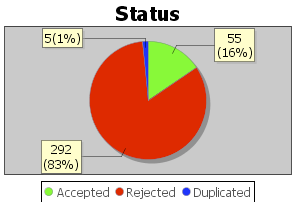
\includegraphics[width=0.5\textwidth]{resources/analisecorre}
	\end{center}
	\legend{Fonte: própria}
\end{figure}

Os resultados do primeiro filtro da revisão (parcial) da literatura estão ilustrados pelo gráfico na \autoref{fig:stascorr} onde a taxa de aceitação e rejeição dos artigos.